\documentclass[oneside, 11pt]{article}

\usepackage[T1]{fontenc}
\usepackage[utf8]{inputenc}
\usepackage[english]{babel}
\usepackage{enumerate}
\usepackage{isotope}


\usepackage{fouriernc}
\usepackage[detect-all, binary-units, separate-uncertainty=true,
            per-mode=symbol, retain-explicit-plus, retain-unity-mantissa=false]{siunitx}

\usepackage{setspace}
\setstretch{1.2}

\setlength{\parskip}{\smallskipamount}
\setlength{\parindent}{0pt}

\usepackage[headheight=14pt]{geometry}
\geometry{marginparwidth=0.5cm, verbose, a4paper, tmargin=3cm, bmargin=3cm,
          lmargin=2cm, rmargin=2cm}

\usepackage{float}

\usepackage[fleqn]{amsmath}
\numberwithin{equation}{section}
\numberwithin{figure}{section}

\usepackage{graphicx}
\graphicspath{{images/}{../../../images/}}

\usepackage{tikz}
\usetikzlibrary{shapes}
\usetikzlibrary{plotmarks}

\newcounter{Exercise}
\setcounter{Exercise}{1}
\usepackage{xcolor}
\definecolor{shadecolor}{gray}{0.9}
\usepackage{framed}
\usepackage{caption}

\usepackage{url}


\usepackage{fancyhdr}
\pagestyle{fancy}
\fancyhf{}
\rhead{\thepage}
\renewcommand{\footrulewidth}{0pt}
\renewcommand{\headrulewidth}{0pt}

\fancypagestyle{firststyle}
{
    \fancyhf{}
    \rhead{\thepage}
    \cfoot{\includegraphics[height=30pt]{HiSPARClogo}}
    \rfoot{\includegraphics[height=25pt]{CCbysa}}
    \lfoot{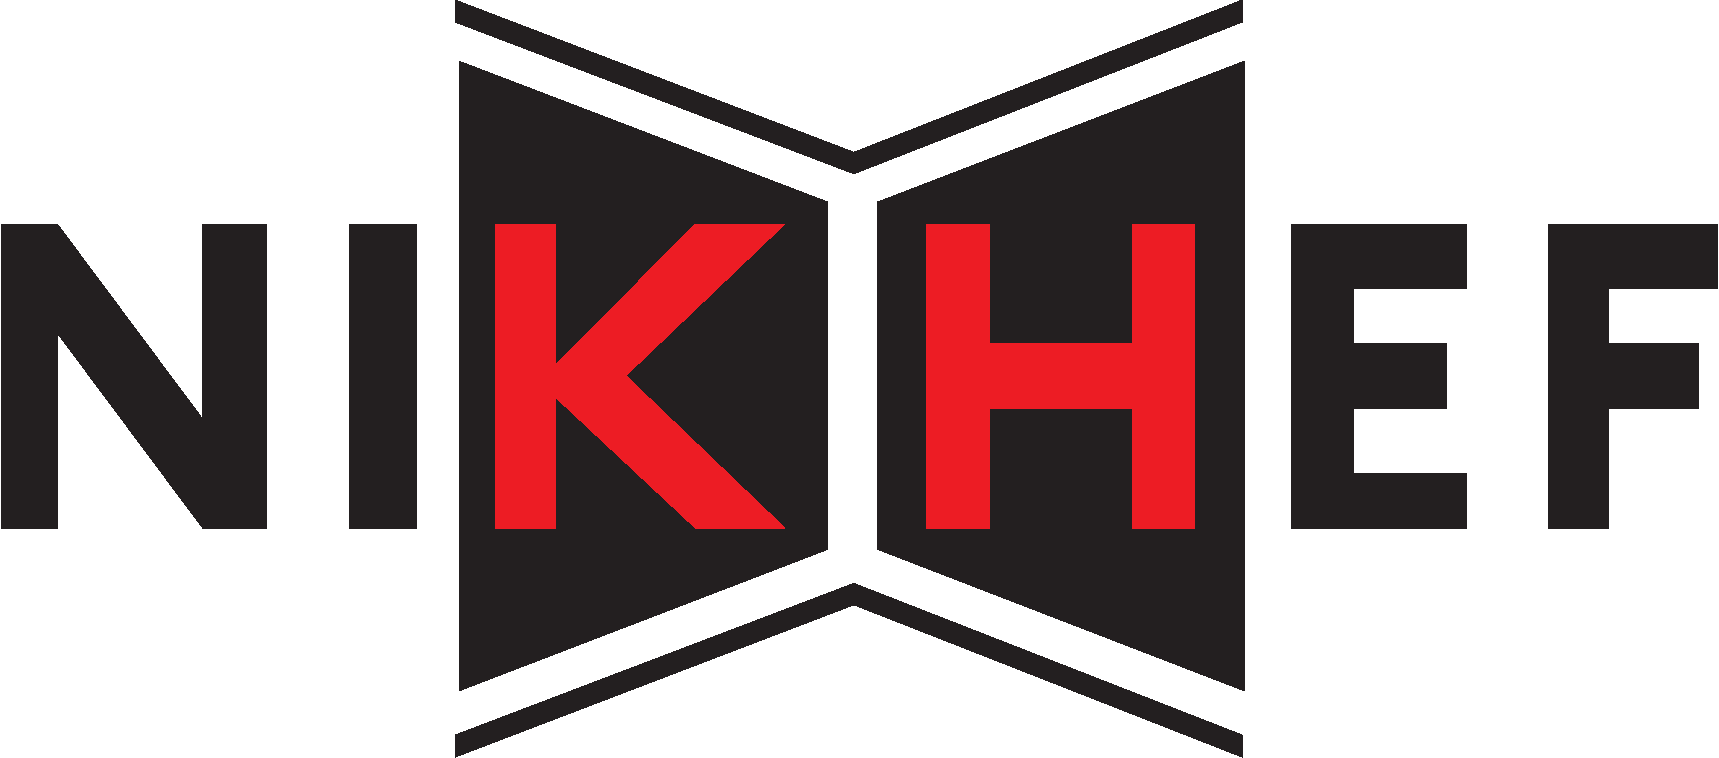
\includegraphics[height=30pt]{NIKHEFlogo}}
    \renewcommand{\footskip}{50pt}
    \renewcommand{\footrulewidth}{0.1pt}
    \renewcommand{\headrulewidth}{0pt}
}

\newcommand{\figref}[1]{Figuur~\ref{#1}}

\newcommand{\hisparc}{\textsmaller{HiSPARC}\xspace}
\newcommand{\kascade}{\textsmaller{KASCADE}\xspace}
\newcommand{\sapphire}{\textsmaller{SAPPHiRE}\xspace}
\newcommand{\jsparc}{\textsmaller{jSparc}\xspace}
\newcommand{\hdf}{\textsmaller{HDF5}\xspace}
\newcommand{\aires}{\textsmaller{AIRES}\xspace}
\newcommand{\csv}{\textsmaller{CSV}\xspace}
\newcommand{\python}{\textsmaller{PYTHON}\xspace}
\newcommand{\corsika}{\textsmaller{CORSIKA}\xspace}
\newcommand{\labview}{\textsmaller{LabVIEW}\xspace}
\newcommand{\daq}{\textsmaller{DAQ}\xspace}
\newcommand{\adc}{\textsmaller{ADC}\xspace}
\newcommand{\hi}{\textsc{h i}\xspace}
\newcommand{\hii}{\textsc{h ii}\xspace}
\newcommand{\mip}{\textsmaller{MIP}\xspace}
\newcommand{\hisparcii}{\textsmaller{HiSPARC II}\xspace}
\newcommand{\hisparciii}{\textsmaller{HiSPARC III}\xspace}

\DeclareSIUnit{\electronvolt}{\ensuremath{\mathrm{e\!\!\:V}}}

\DeclareSIUnit{\unitsigma}{\ensuremath{\sigma}}
\DeclareSIUnit{\mip}{\textsmaller{MIP}}
\DeclareSIUnit{\adc}{\textsmaller{ADC}}

\DeclareSIUnit{\gauss}{G}
\DeclareSIUnit{\parsec}{pc}
\DeclareSIUnit{\year}{yr}



\begin{document}

\title{Parabolische spiegels maken}
\author{N.G. Schultheiss}
\date{}

\maketitle
\thispagestyle{firststyle}

\section{Inleiding}

Deze module volgt op de module ``Spiegels''. Deze module wordt vervolgd
met de module ``Lenzen slijpen''. Uiteindelijk kun je met de opgedane
kennis een telescoop bouwen en de werking verklaren. Deze module is
als een technische module op te vatten. We onderzoeken de technieken
om een parabolische spiegel te maken.

Hieronder volgt een korte samenvatting van de formules die je al beheerst.

\[
v=\frac{\triangle s}{\triangle t}
\]


\[
a=\frac{\Delta v}{\Delta t}
\]


\[
F=m.a
\]


$v$: snelheid (velocity / vitesse) in {[}m/s{]}.

$s$: plaats (space / espace) in {[}m{]}. ($\triangle:$ ``de verandering
van'', bijvoorbeeld $\triangle s=s_{eind}-s_{begin}$.)

$t$: tijd (time / temp) in {[}s{]}.

$a$: versnelling (acceleration) in {[}$\mathrm{m/s^{2}}${]}.

$F$: kracht (force) in {[}N{]}.\newpage{}


\section{Een draaiend vat}

Als we een vloeistof in een draaiend vat gieten krijgt het oppervlak
de vorm van een parabool. Om dit te verklaren bestuderen we eerst
de krachten die bij het draaien optreden. Laten we eerst een soort
kaart van de cirkelbeweging maken voor de tijdstippen $t_{1}$, $t_{2}$,
$t_{3}$ en $t_{4}$.

\begin{figure}[H]
\noindent \begin{centering}
\includegraphics[scale=0.75]{plaats}
\par\end{centering}

\caption{De plaats van een draaiend voorwerp}
\end{figure}


Met figuur 1.1 kunnen we de snelheid bepalen als we de omlooptijd
voor 1 rondje op $T$ zetten. De afgelegde weg kunnen we vinden door
de omtrek van de cirkel door de tijd te delen:

\begin{equation}
v=\frac{2\pi r}{T}
\end{equation}


En ook:

\begin{equation}
T=\frac{2\pi r}{v}
\end{equation}


Figuur 1.1 is een afbeelding een ``plaatsruimte''. We kunnen de
snelheidsvectoren ook in een ``snelheidsruimte'' afbeelden.

\begin{figure}[H]
\noindent \begin{centering}
\includegraphics[scale=0.75]{snelheid}
\par\end{centering}

\caption{De snelheid van een draaiend voorwerp}
\end{figure}


Met figuur 1.1 kunnen we de versnelling bepalen, de omlooptijd is
nog steeds $T$. De snelheidsverandering kunnen we vinden door de
omtrek van de cirkel door de tijd te delen:

\begin{equation}
a=\frac{2\pi v}{T}
\end{equation}


Formule 2.2 is te substitueren in formule 2.3.
\begin{equation}
a=\frac{2\pi v}{(\frac{2\pi r}{v})}
\end{equation}


Of ook:
\begin{equation}
a=\frac{2\pi v^{2}}{2\pi r}
\end{equation}


\begin{equation}
a=\frac{v^{2}}{r}
\end{equation}


We weten dat:

\begin{equation}
F=m.a
\end{equation}


Substitutie geeft:

\begin{equation}
F=\frac{mv^{2}}{r}
\end{equation}


Een draaiend vat verdraaid voor alle punten altijd een zelfde hoek. De
snelheid van een punt en de straal van het punt zijn rechtevenredig. We
introduceren een nieuwe grootheid de hoeksnelheid $\omega$. Deze kan in
graden per seconde, maar liever in radialen \footnote{Een cirkel heeft
$360^{o}$ of $2\pi$ radialen. 1 radiaal is dus $\frac{360^{o}}{2\pi}$.}
per seconde worden gemeten. We kunnen de relatie tussen $v$ en $\omega$
schrijven als: \begin{equation} v=\omega r \end{equation}


Deze middelpuntzoekende kracht is nu ook te schrijven als:

\begin{equation}
F=m\omega^{2}r
\end{equation}


Nu kunnen we schetsen hoe de krachten op een deeltje op het draaiend
vloeistofoppervlak werken. Naast de opwaartse kracht werkt er ook
een middelpuntzoekende kracht op het deeltje.

\begin{figure}[H]
\noindent \begin{centering}
\includegraphics[scale=0.75]{glas}
\par\end{centering}

\caption{De krachten op een deeltje op een draaiend vloeistofoppervlak}
\end{figure}



\paragraph*{Opdracht 1:}

\emph{Bestudeer de afleiding. Probeer te begrijpen hoe de gedachten
zich van formule naar formule ontwikkelen.}


\paragraph*{Opdracht 2:}

\emph{Laat met een schets zien dat de draaiende vloeistof een parabolisch
oppervlak krijgt. }


\section{Glas}

Een draaiend glaasje op een tafel is nog geen spiegel. We hebben nu
echter wel een model hoe we een parabolische spiegel kunnen maken.
Als we een vloeistof kunnen laten stollen hebben we een parabolisch
oppervlak. Een heel vat glas stolt niet overal tegelijk en er ontstaan
spanningen in het glas omdat sommige delen al gestold zijn en al krimpen
terwijl andere delen nog vloeibaar zijn. Deze spanningen zijn te verminderen
door het glas langzaam af te koelen.

Tegenwoordig wordt vensterglas gemaakt met het Pilkington proces.
Bij het Pilkington Float Glass proces laat men het vloeibare glas
op vloeibaar tin stromen. De temperatuur van het tin ligt net onder
het smeltpunt van glas. Aan de ene kant is het glas dus nog vloeibaar
en terwijl het over de tin stroomt stolt het glas. Op een gegeven
moment is het glas vast en kan men de glasplaat van het tinbad afschuiven.
Omdat er steeds nieuw vloeibaar glas wordt aangevoerd kan er in principe
een oneindig lange glasplaat worden gemaakt.

Op vergelijkbare manier kunnen we dus een vat vloeibare tin nemen
en daar een laagje glas op gieten. Na het afkoelen hebben we een parabolische
glasplaat. Dit is natuurlijk een beetje moeilijk thuis of op school
uit te voeren. Met warm water en kaarsvet is dit wel te doen in een
Petri-schaaltje op een draaiend tafeltje.


\paragraph*{Opdracht 3:}

\emph{Probeer met water en paraffine (kaarsvet) een werkend productieproces
voor parabolische oppervlakken te maken. Maak een verslag van je onderzoek.
Wat heb je nodig? Hoe werkt het proces? Wat zijn de problemen? Hoe
los je die op?}


\paragraph*{Opdracht 4:}

\emph{Om spiegels te maken moeten we omschakelen van water met paraffine
naar tin en glas. Deze stoffen moeten redelijk zuiver zijn om een
homogene spiegel te maken. Onderzoek hoe glas gemaakt wordt.}

\end{document}
